% !TEX root = thesis.tex
\chapter{はじめに}
\label{chap:preface}
\section{ウェブ工学と機械学習}
ウェブ工学の領域においては、様々な知識をプログラムに学習させ、これによって物事の予測や分類を行うことが求められている。例えば、ウェブサイトを閲覧しているユーザに商品や広告を提示するとき、ユーザが購入したい商品をプログラムに予測させることが出来れば、ユーザの購買行動を促進できる。この技術は推薦システムと呼ばれている\cite{resnick1997recommender}。また、検索エンジンを作るときは、ユーザが求めている情報をより的確に予測して、出来るだけ無駄無く取りこぼしも少なく表示させたい。この予測技術は、Learng to Rankと呼ばれている\cite{trotman2005learning}。こういった知識学習と予測・分類のためには、機械学習(Machine Learning)と呼ばれる手法が広く用いられている。\par
機械学習とは、対象となる知識を数学的なモデルで表し、より適切なモデルを求めて微修正を重ねることで、知識を洗練させていくアプローチである。使用する数学的なモデルの大筋は、経験を基にあらかじめ決めておく。ユーザ行動、リンク構造、メールの文章といった元データは、全て数値に変換されて、モデルに入力される。モデルは、入力データから予測や識別を実際に行いつつ、より良い結果が得られるように、モデル内の係数を調整していく。最終的に、多種多様なデータに対して、適切な予測や識別を行うことが出来る数学的モデルを得ることができるのである。

\section{深層学習の台頭}
機械学習における大きなポイントの1つに、元データをどのような数値データに変換するか、という問題がある。\par
機械学習の一般的なプロセスを、図\ref{c1_ml}に示す。変換された数値データのことを、 特徴量、あるいは素性(feature)と呼ぶ。機械学習は、「生データから素性への変換」「素性をモデルに入力」「モデルによる数値計算で、結果を出力」「結果がより正確になるよう、モデルを修正」というプロセスの繰り返しで成り立っている。このうち、「素性への変換」だけは、画像・文章・リンク構造といった、データの種類に依存している。いったん素性が数値の形で得られれば、残りのプロセスは、データの種類に依存せず、全て入力数値とモデルの関係だけで解決することができる。つまり、機械学習のプロセスは、データの種類に依存する素性変換と、汎用的に使えるモデル学習の部分に分かれているのである。
\begin{figure}[tbp]
 \centering
  
\includegraphics[width=80mm]{img/c1/ml}
 \caption{機械学習の一般的プロセス(\cite{bishop2006pattern}を基に作成)}
 \label{c1_ml}
\end{figure}
\par
機械学習の性能を上げるためには、素性への変換部分を工夫する方法と、使用する数学的モデルを洗練する方法の2つがある。素性への変換部分の改良は、対象となるデータの種類に強く依存している。例えば、画像データを素性数値に変換する場合、単純なRGB画素データをそのまま使っても良いが、SIFT特徴量\cite{lowe1999object}やSURF特徴量\cite{bay2008speeded-up}、フィッシャーベクトル\cite{perronnin2007fisher}など、より画像の特徴を捉えた特徴量を用いることが定石となっている。音声データに対しては、時間領域や周波数領域の波形をそのまま用いることもあるが、他にメル周波数ケプストラム係数などの特徴量も使われる\cite{logan2000mel-frequency}。問題とデータ種別に応じて、利用する特徴量を工夫することにより、機械学習の識別精度や実行時間などの性能が向上することが知られている。\par
従来、特徴量は画像や音声などそれぞれのデータの専門家による、謂わば職人芸によって作られていた。その後2000年代半ばに、深層学習(Deep Learning)と呼ばれる一群の手法が台頭した。深層学習とは機械学習の手法の1つで、人間の脳の構造に類似した、多層ニューラルネットワーク構造をモデルに用いて、学習を行わせる方法である。深層学習には、今まで専門家によって行われてきた特徴量の変換方法それ自体も、習得する能力があると考えられている。生のデータを入力して学習させると、データから自動的に素性を作り、抽象表現を習得することが出来るようになるのである。この深層学習は、画像認識や音声認識、化合物の生成予測といった分野で優れた性能を示し、注目を浴びるようになった。図\ref{c1_nikkei}は、多層ニューラルネットワークが人間の脳の思考回路である、神経細胞のつながりを模倣する様子を表している。\par
%注目の表現で、googleやnips2013の様子、buyoutなど
\begin{figure}[tbp]
 \begin{center}
  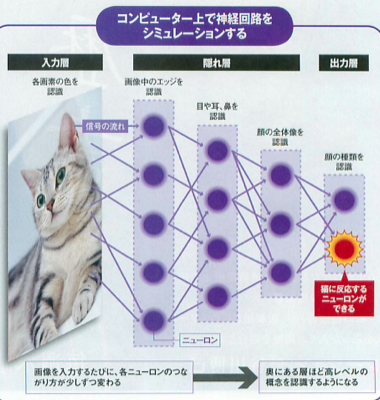
\includegraphics[width=80mm]{img/c1/nikkei}
 \end{center}
 \caption{深層学習で画像を認識する流れ (日経ビジネス2013年4月号より一部抜粋)}
 \label{c1_nikkei}
\end{figure}
深層学習の特徴の一つである、素性学習について、詳しく述べる。例えば人間の顔画像データを学習させた場合、多層ニューラルネットワークを構成する複数のレイヤーのうち、入力に近い低レイヤーのニューロンは、画像のエッジ部分に対して強く反応し、出力に近い高レイヤーのニューロンでは、目口鼻、さらに顔全体など、より抽象度の高い要素に対して反応することがわかった。これは、見方を変えれば、低レイヤーでは中間表現(素性にあたる)を抽出しており、低レイヤーで得た素性を高レイヤーに入力することにより、より高レベルな抽象的概念に対しても優れた識別精度を実現している、と考えられる。どのような素性を使えば良い結果が出るのか、素性の抽出方法自体を同時に機械学習していることから、深層学習は表現学習(Representation Learning)とも呼ばれている。\par
図\ref{c1_lee2009_faces}は、2009年、LeeらによるConvolutional Deep Belief Networkの実験によって学習された顔の要素である\cite{lee2009convolutional}。上が2レイヤー目、下が3レイヤー目で、2レイヤー目では、鼻や口、目といった顔を構成するパーツが学習されている。これは、単なる画素の数値に比べて、明らかに抽象度の高い情報に反応していると言える。さらに、3レイヤー目では人間の顔を学習することに成功している。2レイヤー目で作り出した、「顔のパーツ」という素性を元にして、さらに抽象度の高い、人間の顔という要素を推論しているのである。
\begin{figure}[tbp]
 \centering
  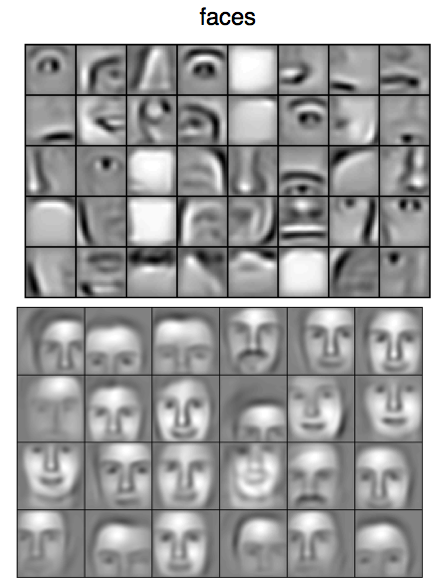
\includegraphics[width=80mm]{img/c1/lee2009_faces}
 \caption{深層学習による、顔の構成要素の学習結果(\cite{lee2009convolutional}より引用)}
 \label{c1_lee2009_faces}
\end{figure}
\par

Googleの深層学習研究グループは2012年、Youtubeのビデオから抽出した静止画による教師無し学習によって、人間や猫の顔画像を識別できる多層ニューラルネットワークモデルの学習に成功し、大きな話題を呼んだ\cite{le2012building}。\par
\begin{figure}[tbp]
 \begin{center}
  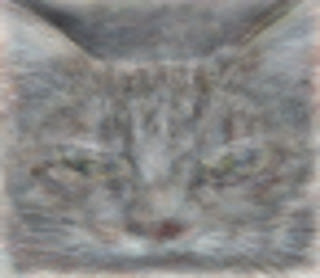
\includegraphics[width=50mm]{img/c1/cat_detection}
 \end{center}
 \caption{猫の画像に反応するニューロン (\cite{le2012building}より引用)}
 \label{c1_catdetection}
\end{figure}

\begin{figure}[tbp]
 \begin{center}
  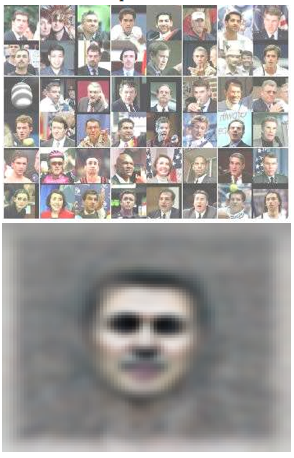
\includegraphics[width=50mm]{img/c1/google_face}
 \end{center}
 \caption{上 : 入力画像の中で、ニューロンが最も強く反応した48枚。下 : 計算上、最もニューロンが強く反応する画像\newline  (Googleの研究紹介記事より引用。http://googleblog.blogspot.jp/2012/06/using-large-scale-brain-simulations-for.html)}%
 
 \label{c1_facedetection}
\end{figure}


\section{深層学習の課題と、研究の目的}
深層学習が高い識別性能を持つことがわかり、深層学習を身近な問題に適用して、良い成果を得たいという機運が高まっている。例えば、ウェブ工学の分野では機械学習が大きな役割を果たしており、この学習プロセスに深層学習を組みこむことで、学習精度が向上したり、より多様な情報を扱えるようになる可能性がある。出来るだけ簡易に、深層学習を様々な問題に応用するための方法論が求められている。\par
しかし、深層学習は歴史の浅い発展途上の技術であり、そもそも正しい実装を行って論文同様の分類精度を発揮すること自体が難しい。また、学習時間が長く大きなマシンパワーが必要になることが多い。原理が複雑で実世界での応用例もまだ少ないため、プログラム開発に長い時間がかかってしまう。つまり、ウェブ工学など応用分野に深層学習を適用したいと考えても、実際の問題に深層学習を試行して結果を出すこと自体が困難であり、応用技術開発のハードルは更に高くなってしまっている。特に、国内での研究開発は遅れており、早急なキャッチアップが必要である。\par
本研究では、このような現状を踏まえ、深層学習技術をウェブ工学など実際の問題に応用するために、「分類精度の再現の問題」「学習時間の問題」「実装難易度の問題」という3つの応用上の問題点に注目し、これを出来る限り緩和するための方策を提案する。まず、3つの問題点全てに適用できる対策として、適切な深層学習ライブラリの選択が有効であることを示す。また、「学習時間の問題」については、Graphics Processing Unit(以下GPU)の使用が有効であることも示す。その上で、今現在利用可能な深層学習ライブラリを比較し、Pylearn2とDeep Learning Tutorialという2つのライブラリが、問題点のうち「学習時間の問題」「実装難易度の問題」の2つを解決することを示す。さらに、この2つのライブラリに実装されている深層学習のモデルにより、分類精度の再現実験を行い、「分類精度の再現の問題」が解決できることを検証する。\par
2章では、従来のウェブ工学における機械学習の応用方法と、深層学習出現以前に良く用いられていた、機械学習による識別器学習方法について、俯瞰する。3章では、深層学習を構成する個々のアルゴリズムについて、その原理と詳細を述べる。4章では、実際に深層学習アルゴリズムを利用する上で、どのように実装を進めれば、先に上げた問題点を緩和できるのかを述べる。5章では、深層学習のプログラムを、汎用的なベンチマークにかけることで、その性能を測定・比較する。6章では、5章までの結果を受けて、深層学習を利用していく上でのベストプラクティスを考察する。
